\chapter{Learning from complex vehicle model}
\label{cha:Tracking_MPC}

%Plot simulink model en duidt de blokken aan die zullen worden ingevuld. Hier gaat dieper in gegaan worden in de volgende hoofdstukken. 

Because the non-linear bicycle model makes abstraction of dynamics that are applicable in a real vehicle, a more complex model is introduced in order to improve the reality factor of the simulations. In order to achieve this the $15$ degrees of freedom amesim model as is seen in Figure \ref{fig:Amesim}, is provided by Siemens. The parameters of this model are tuned by the company in order to behave similar to a testcar they are currently using. The model has as inputs the amount of throttle, braking and an steerwheelangle.

\begin{figure}[h!]
	\centering
	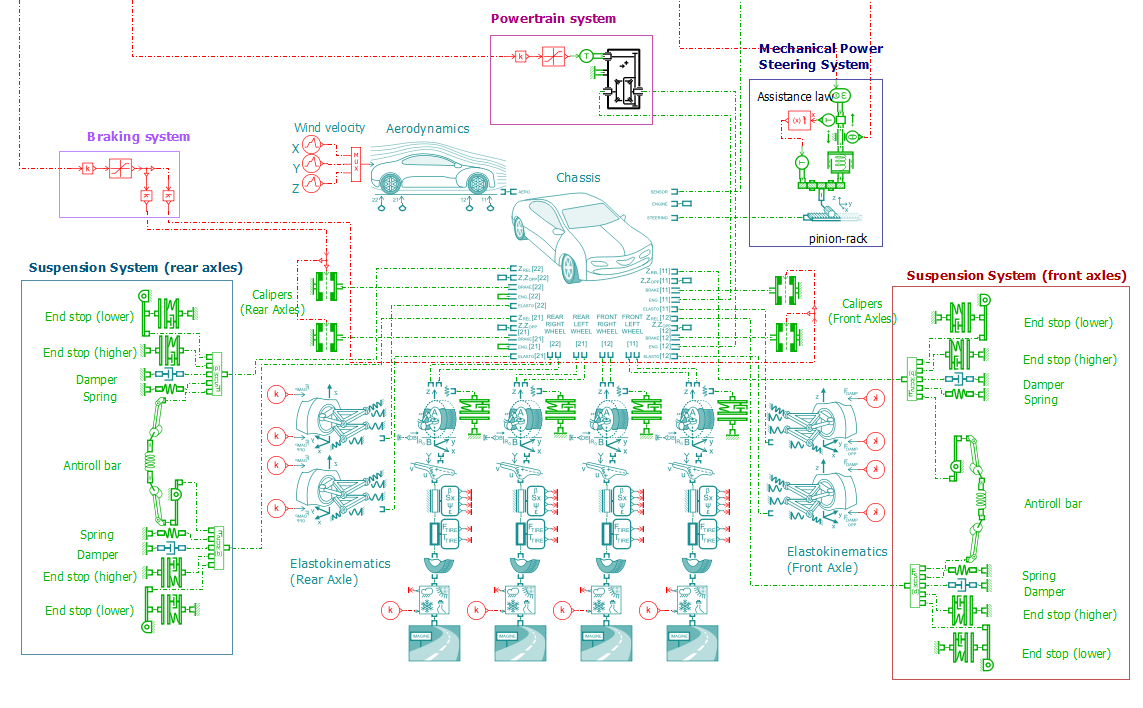
\includegraphics[width=1.0\textwidth]{Amesim.PNG}
	\label{fig:Amesim}
	\caption{The 15 dof amesim model with as inputs the amount of throtttle, braking and steerwheelangle.}	
\end{figure}


The way how the amesim model is integrated in the learning algorithm can be seen in Figure \ref{fig:complex_learning}. 

\begin{figure}[h!]
	\centering
	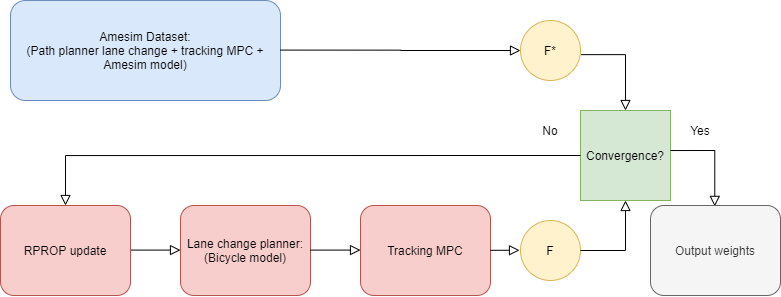
\includegraphics[width=1.1\textwidth]{complex_learning_diagram.PNG}
	\label{fig:Amesim}
	\caption{The 15 dof amesim model with as inputs the amount of throtttle, braking and steerwheelangle.}	
\end{figure}
 
\section{The First Topic of this Chapter}
\subsection{Item 1}
\subsubsection{Sub-item 1}


\subsubsection{Sub-item 2}


\subsection{Item 2}


\section{The Second Topic}


\section{Conclusion}

%%% Local Variables: 
%%% mode: latex
%%% TeX-master: "thesis"
%%% End: 